\documentclass[tikz]{standalone}

\usepackage{amsmath}
\usepackage{tikz}
%\usepackage{etoolbox}
\usepackage{listofitems}
\usetikzlibrary{arrows.meta}
\usepackage[outline]{contour}
\contourlength{1.4pt}

\tikzset{>=latex}
\usepackage{xcolor}

\tikzstyle{node}=[circle,draw=black,minimum size=22,inner sep=0.5,outer sep=0.6]

\tikzstyle{node in}=[node,green!20!black,draw=black,fill=orange!50]
\tikzstyle{node hidden}=[node,blue!20!black,draw=black,fill=lime!50]
\tikzstyle{node out}=[node,red!20!black,draw=black,fill=yellow!50]

\tikzstyle{connect arrow}=[-{Latex[length=3,width=3]},black,shorten <=0.5,shorten >=1]
\tikzset{
  node 1/.style={node in},
  node 2/.style={node hidden},
  node 3/.style={node out},
}
\def\nstyle{int(\lay<\Nnodlen?min(2,\lay):3)}


\begin{document}

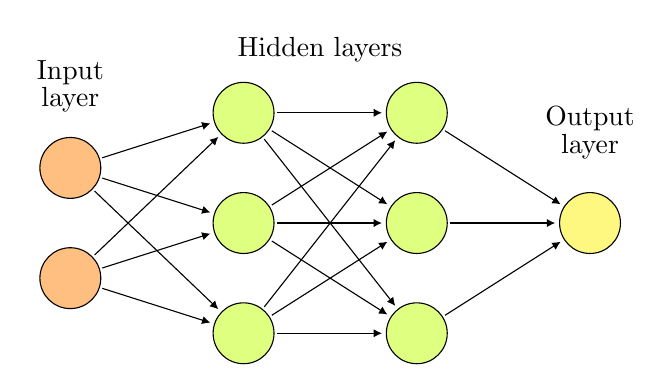
\begin{tikzpicture}[x=2.2cm,y=1.4cm]
  \readlist\Nnod{2, 3, 3, 1}

  \foreachitem \N \in \Nnod{
    \edef\lay{\Ncnt}
    \message{\lay,}
    \pgfmathsetmacro\prev{int(\Ncnt-1)}
    \foreach \i [evaluate={\y=\N/2-\i; \x=\lay; \n=\nstyle;}] in {1,...,\N}{

      % nodes
      \node[node \n] (N\lay-\i) at (\x,\y) {};

      % edges
      \ifnum\lay>1
        \foreach \j in {1,...,\Nnod[\prev]}{
          \draw[connect arrow] (N\prev-\j) -- (N\lay-\i);
        }
      \fi

    }

  }

  % labels
  \node[above=5,align=center,black] at (N1-1.90) {Input\\[-0.2em]layer};
  \node[above of = 2, above=-0.6cm, align=center,black, right=-0.2cm] at (N2-1.90) {Hidden layers};
  \node[above=8,align=center,black] at (N\Nnodlen-1.90) {Output\\[-0.2em]layer};

\end{tikzpicture}

\end{document}